% Options for packages loaded elsewhere
\PassOptionsToPackage{unicode}{hyperref}
\PassOptionsToPackage{hyphens}{url}
%
\documentclass[
]{article}
\title{First project John Hopkins}
\author{Akanksha}
\date{2/22/2022}

\usepackage{amsmath,amssymb}
\usepackage{lmodern}
\usepackage{iftex}
\ifPDFTeX
  \usepackage[T1]{fontenc}
  \usepackage[utf8]{inputenc}
  \usepackage{textcomp} % provide euro and other symbols
\else % if luatex or xetex
  \usepackage{unicode-math}
  \defaultfontfeatures{Scale=MatchLowercase}
  \defaultfontfeatures[\rmfamily]{Ligatures=TeX,Scale=1}
\fi
% Use upquote if available, for straight quotes in verbatim environments
\IfFileExists{upquote.sty}{\usepackage{upquote}}{}
\IfFileExists{microtype.sty}{% use microtype if available
  \usepackage[]{microtype}
  \UseMicrotypeSet[protrusion]{basicmath} % disable protrusion for tt fonts
}{}
\makeatletter
\@ifundefined{KOMAClassName}{% if non-KOMA class
  \IfFileExists{parskip.sty}{%
    \usepackage{parskip}
  }{% else
    \setlength{\parindent}{0pt}
    \setlength{\parskip}{6pt plus 2pt minus 1pt}}
}{% if KOMA class
  \KOMAoptions{parskip=half}}
\makeatother
\usepackage{xcolor}
\IfFileExists{xurl.sty}{\usepackage{xurl}}{} % add URL line breaks if available
\IfFileExists{bookmark.sty}{\usepackage{bookmark}}{\usepackage{hyperref}}
\hypersetup{
  pdftitle={First project John Hopkins},
  pdfauthor={Akanksha},
  hidelinks,
  pdfcreator={LaTeX via pandoc}}
\urlstyle{same} % disable monospaced font for URLs
\usepackage[margin=1in]{geometry}
\usepackage{color}
\usepackage{fancyvrb}
\newcommand{\VerbBar}{|}
\newcommand{\VERB}{\Verb[commandchars=\\\{\}]}
\DefineVerbatimEnvironment{Highlighting}{Verbatim}{commandchars=\\\{\}}
% Add ',fontsize=\small' for more characters per line
\usepackage{framed}
\definecolor{shadecolor}{RGB}{248,248,248}
\newenvironment{Shaded}{\begin{snugshade}}{\end{snugshade}}
\newcommand{\AlertTok}[1]{\textcolor[rgb]{0.94,0.16,0.16}{#1}}
\newcommand{\AnnotationTok}[1]{\textcolor[rgb]{0.56,0.35,0.01}{\textbf{\textit{#1}}}}
\newcommand{\AttributeTok}[1]{\textcolor[rgb]{0.77,0.63,0.00}{#1}}
\newcommand{\BaseNTok}[1]{\textcolor[rgb]{0.00,0.00,0.81}{#1}}
\newcommand{\BuiltInTok}[1]{#1}
\newcommand{\CharTok}[1]{\textcolor[rgb]{0.31,0.60,0.02}{#1}}
\newcommand{\CommentTok}[1]{\textcolor[rgb]{0.56,0.35,0.01}{\textit{#1}}}
\newcommand{\CommentVarTok}[1]{\textcolor[rgb]{0.56,0.35,0.01}{\textbf{\textit{#1}}}}
\newcommand{\ConstantTok}[1]{\textcolor[rgb]{0.00,0.00,0.00}{#1}}
\newcommand{\ControlFlowTok}[1]{\textcolor[rgb]{0.13,0.29,0.53}{\textbf{#1}}}
\newcommand{\DataTypeTok}[1]{\textcolor[rgb]{0.13,0.29,0.53}{#1}}
\newcommand{\DecValTok}[1]{\textcolor[rgb]{0.00,0.00,0.81}{#1}}
\newcommand{\DocumentationTok}[1]{\textcolor[rgb]{0.56,0.35,0.01}{\textbf{\textit{#1}}}}
\newcommand{\ErrorTok}[1]{\textcolor[rgb]{0.64,0.00,0.00}{\textbf{#1}}}
\newcommand{\ExtensionTok}[1]{#1}
\newcommand{\FloatTok}[1]{\textcolor[rgb]{0.00,0.00,0.81}{#1}}
\newcommand{\FunctionTok}[1]{\textcolor[rgb]{0.00,0.00,0.00}{#1}}
\newcommand{\ImportTok}[1]{#1}
\newcommand{\InformationTok}[1]{\textcolor[rgb]{0.56,0.35,0.01}{\textbf{\textit{#1}}}}
\newcommand{\KeywordTok}[1]{\textcolor[rgb]{0.13,0.29,0.53}{\textbf{#1}}}
\newcommand{\NormalTok}[1]{#1}
\newcommand{\OperatorTok}[1]{\textcolor[rgb]{0.81,0.36,0.00}{\textbf{#1}}}
\newcommand{\OtherTok}[1]{\textcolor[rgb]{0.56,0.35,0.01}{#1}}
\newcommand{\PreprocessorTok}[1]{\textcolor[rgb]{0.56,0.35,0.01}{\textit{#1}}}
\newcommand{\RegionMarkerTok}[1]{#1}
\newcommand{\SpecialCharTok}[1]{\textcolor[rgb]{0.00,0.00,0.00}{#1}}
\newcommand{\SpecialStringTok}[1]{\textcolor[rgb]{0.31,0.60,0.02}{#1}}
\newcommand{\StringTok}[1]{\textcolor[rgb]{0.31,0.60,0.02}{#1}}
\newcommand{\VariableTok}[1]{\textcolor[rgb]{0.00,0.00,0.00}{#1}}
\newcommand{\VerbatimStringTok}[1]{\textcolor[rgb]{0.31,0.60,0.02}{#1}}
\newcommand{\WarningTok}[1]{\textcolor[rgb]{0.56,0.35,0.01}{\textbf{\textit{#1}}}}
\usepackage{graphicx}
\makeatletter
\def\maxwidth{\ifdim\Gin@nat@width>\linewidth\linewidth\else\Gin@nat@width\fi}
\def\maxheight{\ifdim\Gin@nat@height>\textheight\textheight\else\Gin@nat@height\fi}
\makeatother
% Scale images if necessary, so that they will not overflow the page
% margins by default, and it is still possible to overwrite the defaults
% using explicit options in \includegraphics[width, height, ...]{}
\setkeys{Gin}{width=\maxwidth,height=\maxheight,keepaspectratio}
% Set default figure placement to htbp
\makeatletter
\def\fps@figure{htbp}
\makeatother
\setlength{\emergencystretch}{3em} % prevent overfull lines
\providecommand{\tightlist}{%
  \setlength{\itemsep}{0pt}\setlength{\parskip}{0pt}}
\setcounter{secnumdepth}{-\maxdimen} % remove section numbering
\ifLuaTeX
  \usepackage{selnolig}  % disable illegal ligatures
\fi

\begin{document}
\maketitle

Lets begin with step 1 and read the data here.

\begin{Shaded}
\begin{Highlighting}[]
\NormalTok{df }\OtherTok{\textless{}{-}} \FunctionTok{read.csv}\NormalTok{(}\StringTok{"activity.csv"}\NormalTok{ , }\AttributeTok{header =} \ConstantTok{TRUE}\NormalTok{)}
\DocumentationTok{\#\#Taking a sneak peak inside data to make sure its read correctly.}
\FunctionTok{head}\NormalTok{(df)}
\end{Highlighting}
\end{Shaded}

\begin{verbatim}
##   steps       date interval
## 1    NA 2012-10-01        0
## 2    NA 2012-10-01        5
## 3    NA 2012-10-01       10
## 4    NA 2012-10-01       15
## 5    NA 2012-10-01       20
## 6    NA 2012-10-01       25
\end{verbatim}

For a better understanding of data, we can see its glimpse using the
glimpse function. we would need to load Tidyverse package in order to
use this fucntion

\begin{Shaded}
\begin{Highlighting}[]
\FunctionTok{library}\NormalTok{(tidyverse)}
\end{Highlighting}
\end{Shaded}

\begin{verbatim}
## -- Attaching packages --------------------------------------- tidyverse 1.3.1 --
\end{verbatim}

\begin{verbatim}
## v ggplot2 3.3.5     v purrr   0.3.4
## v tibble  3.1.6     v dplyr   1.0.7
## v tidyr   1.1.4     v stringr 1.4.0
## v readr   2.1.1     v forcats 0.5.1
\end{verbatim}

\begin{verbatim}
## -- Conflicts ------------------------------------------ tidyverse_conflicts() --
## x dplyr::filter() masks stats::filter()
## x dplyr::lag()    masks stats::lag()
\end{verbatim}

\begin{Shaded}
\begin{Highlighting}[]
\FunctionTok{glimpse}\NormalTok{(df)}
\end{Highlighting}
\end{Shaded}

\begin{verbatim}
## Rows: 17,568
## Columns: 3
## $ steps    <int> NA, NA, NA, NA, NA, NA, NA, NA, NA, NA, NA, NA, NA, NA, NA, N~
## $ date     <chr> "2012-10-01", "2012-10-01", "2012-10-01", "2012-10-01", "2012~
## $ interval <int> 0, 5, 10, 15, 20, 25, 30, 35, 40, 45, 50, 55, 100, 105, 110, ~
\end{verbatim}

we notice that date column of the dataset is ``character'' type. we need
to change this using lubridate package and converting it into date type.

\begin{Shaded}
\begin{Highlighting}[]
\FunctionTok{library}\NormalTok{(lubridate)}
\end{Highlighting}
\end{Shaded}

\begin{verbatim}
## 
## Attaching package: 'lubridate'
\end{verbatim}

\begin{verbatim}
## The following objects are masked from 'package:base':
## 
##     date, intersect, setdiff, union
\end{verbatim}

\begin{Shaded}
\begin{Highlighting}[]
\NormalTok{df}\SpecialCharTok{$}\NormalTok{date }\OtherTok{\textless{}{-}} \FunctionTok{ymd}\NormalTok{(df}\SpecialCharTok{$}\NormalTok{date)}
\end{Highlighting}
\end{Shaded}

To begin with the code for step 2 , plotting Histogram of total number
of steps taken each day , we first need to calculate the total steps for
each day.

\begin{Shaded}
\begin{Highlighting}[]
\NormalTok{histdf }\OtherTok{\textless{}{-}}\NormalTok{ df}\SpecialCharTok{\%\textgreater{}\%}\FunctionTok{group\_by}\NormalTok{(date)}\SpecialCharTok{\%\textgreater{}\%}\FunctionTok{summarise}\NormalTok{(}\StringTok{"total\_steps"} \OtherTok{=} \FunctionTok{sum}\NormalTok{(steps))}
\FunctionTok{head}\NormalTok{(histdf)}
\end{Highlighting}
\end{Shaded}

\begin{verbatim}
## # A tibble: 6 x 2
##   date       total_steps
##   <date>           <int>
## 1 2012-10-01          NA
## 2 2012-10-02         126
## 3 2012-10-03       11352
## 4 2012-10-04       12116
## 5 2012-10-05       13294
## 6 2012-10-06       15420
\end{verbatim}

Here we get a tibble object displaying the summarised data where each
date is followed by a column stating the total steps taken on that day.
Now we will proceed with the histogram.

\begin{Shaded}
\begin{Highlighting}[]
\FunctionTok{hist}\NormalTok{(histdf}\SpecialCharTok{$}\NormalTok{total\_steps, }\AttributeTok{xlab =} \StringTok{"total steps"}\NormalTok{, }\AttributeTok{main =} \StringTok{"Histogram of the total number of steps taken each day"}\NormalTok{ , }\AttributeTok{col =} \StringTok{"orange"}\NormalTok{)}
\end{Highlighting}
\end{Shaded}

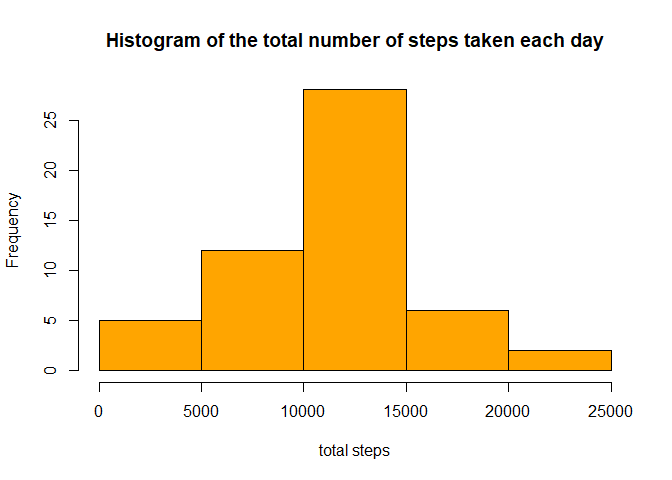
\includegraphics{PA1_template_files/figure-latex/unnamed-chunk-5-1.pdf}
For step 3, we can use Tidyverse package to summarise data in terms of
mean and median.

\begin{Shaded}
\begin{Highlighting}[]
\NormalTok{dfstep3 }\OtherTok{\textless{}{-}}\NormalTok{ df}\SpecialCharTok{\%\textgreater{}\%}\FunctionTok{group\_by}\NormalTok{(date)}\SpecialCharTok{\%\textgreater{}\%}\FunctionTok{summarise}\NormalTok{(}\StringTok{"mean\_steps"} \OtherTok{=} \FunctionTok{mean}\NormalTok{(steps)}
\NormalTok{                                           ,}\StringTok{"median\_steps"} \OtherTok{=} \FunctionTok{median}\NormalTok{(steps))}
\FunctionTok{head}\NormalTok{(dfstep3)}
\end{Highlighting}
\end{Shaded}

\begin{verbatim}
## # A tibble: 6 x 3
##   date       mean_steps median_steps
##   <date>          <dbl>        <dbl>
## 1 2012-10-01     NA               NA
## 2 2012-10-02      0.438            0
## 3 2012-10-03     39.4              0
## 4 2012-10-04     42.1              0
## 5 2012-10-05     46.2              0
## 6 2012-10-06     53.5              0
\end{verbatim}

Here we proceed to next step. First we will summarise average steps for
each interval across all days, then we will proceed with it's plot.

\begin{Shaded}
\begin{Highlighting}[]
\NormalTok{dfstep4 }\OtherTok{\textless{}{-}}\NormalTok{ df}\SpecialCharTok{\%\textgreater{}\%}\FunctionTok{group\_by}\NormalTok{(interval,date)}\SpecialCharTok{\%\textgreater{}\%}\FunctionTok{summarise}\NormalTok{(}\StringTok{"avgsteps"} \OtherTok{=} \FunctionTok{mean}\NormalTok{(steps))}
\end{Highlighting}
\end{Shaded}

\begin{verbatim}
## `summarise()` has grouped output by 'interval'. You can override using the `.groups` argument.
\end{verbatim}

\begin{Shaded}
\begin{Highlighting}[]
\FunctionTok{library}\NormalTok{(ggplot2)}
\NormalTok{dfstep4}\SpecialCharTok{\%\textgreater{}\%}\FunctionTok{ggplot}\NormalTok{(}\AttributeTok{mapping =} \FunctionTok{aes}\NormalTok{( }\AttributeTok{x =}\NormalTok{ interval,  }\AttributeTok{y =}\NormalTok{ avgsteps))}\SpecialCharTok{+}
  \FunctionTok{geom\_line}\NormalTok{()}\SpecialCharTok{+}
  \FunctionTok{labs}\NormalTok{( }\AttributeTok{x =} \StringTok{"Interval across all days"}\NormalTok{, }\AttributeTok{y =} \StringTok{"Average steps taken"}\NormalTok{,}\AttributeTok{title =}       \StringTok{"plot for average steps taken in each time interval"}\NormalTok{)}
\end{Highlighting}
\end{Shaded}

\begin{verbatim}
## Warning: Removed 2 row(s) containing missing values (geom_path).
\end{verbatim}

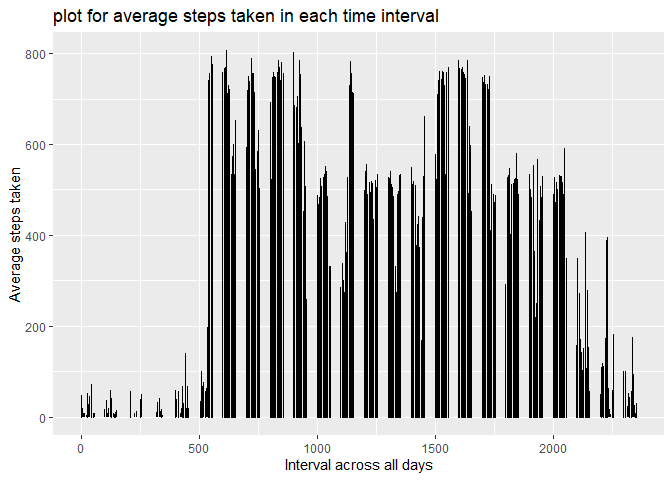
\includegraphics{PA1_template_files/figure-latex/unnamed-chunk-7-1.pdf}
to get the interval containing maximum number of steps, we can make use
of above tibble and calculate max

\begin{Shaded}
\begin{Highlighting}[]
\NormalTok{dfstep4[}\FunctionTok{which.max}\NormalTok{(dfstep4}\SpecialCharTok{$}\NormalTok{avgsteps),]}
\end{Highlighting}
\end{Shaded}

\begin{verbatim}
## # A tibble: 1 x 3
## # Groups:   interval [1]
##   interval date       avgsteps
##      <int> <date>        <dbl>
## 1      615 2012-11-27      806
\end{verbatim}

here we get the interval for which we have maximum number of average
steps.

Now for the next task, we first need to report the total number of
missing values in the dataset

\begin{Shaded}
\begin{Highlighting}[]
\FunctionTok{nrow}\NormalTok{(df[}\SpecialCharTok{!}\FunctionTok{complete.cases}\NormalTok{(df),])}
\end{Highlighting}
\end{Shaded}

\begin{verbatim}
## [1] 2304
\end{verbatim}

we will now devise a strategy to fill all of the NA values and replace
it with 0 instead.

\begin{Shaded}
\begin{Highlighting}[]
\NormalTok{ df}\SpecialCharTok{$}\NormalTok{steps }\OtherTok{\textless{}{-}}\NormalTok{ df}\SpecialCharTok{$}\NormalTok{steps}\SpecialCharTok{\%\textgreater{}\%}\FunctionTok{replace\_na}\NormalTok{(}\StringTok{"0"}\NormalTok{)}
\end{Highlighting}
\end{Shaded}

Now we have a new dataset where all the missing values i.e NA is now
replaced with zero. For the next step of assignment , we will see if
this brings any change to the plots we earlier made.

\begin{Shaded}
\begin{Highlighting}[]
\NormalTok{df}\SpecialCharTok{$}\NormalTok{steps }\OtherTok{\textless{}{-}} \FunctionTok{as.numeric}\NormalTok{(df}\SpecialCharTok{$}\NormalTok{steps)}
\NormalTok{histdf }\OtherTok{\textless{}{-}}\NormalTok{ df}\SpecialCharTok{\%\textgreater{}\%}\FunctionTok{group\_by}\NormalTok{(date)}\SpecialCharTok{\%\textgreater{}\%}\FunctionTok{summarise}\NormalTok{(}\StringTok{"total\_steps"}\OtherTok{=}\NormalTok{(}\FunctionTok{sum}\NormalTok{(steps)))}
\FunctionTok{hist}\NormalTok{(histdf}\SpecialCharTok{$}\NormalTok{total\_steps, }\AttributeTok{xlab =} \StringTok{"total steps"}\NormalTok{, }\AttributeTok{main =} \StringTok{"Histogram of the total number of steps taken each day"}\NormalTok{ , }\AttributeTok{col =} \StringTok{"blue"}\NormalTok{)}
\end{Highlighting}
\end{Shaded}

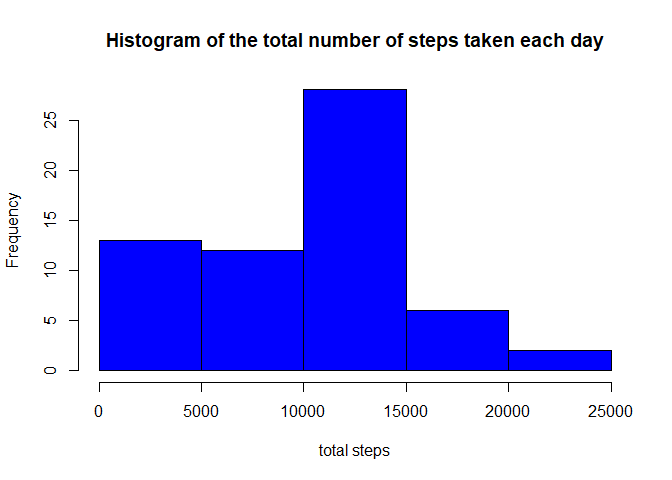
\includegraphics{PA1_template_files/figure-latex/unnamed-chunk-11-1.pdf}
The histogram plotting doesn't seem much changed. We will next check it
for other reportings calculated for mean and median.

\begin{Shaded}
\begin{Highlighting}[]
\NormalTok{dfstep7 }\OtherTok{\textless{}{-}}\NormalTok{ df}\SpecialCharTok{\%\textgreater{}\%}\FunctionTok{group\_by}\NormalTok{(date)}\SpecialCharTok{\%\textgreater{}\%}\FunctionTok{summarise}\NormalTok{(}\StringTok{"mean\_steps"} \OtherTok{=} \FunctionTok{mean}\NormalTok{(steps)}
\NormalTok{                                           ,}\StringTok{"median\_steps"} \OtherTok{=} \FunctionTok{median}\NormalTok{(steps))}
\FunctionTok{head}\NormalTok{(dfstep7)}
\end{Highlighting}
\end{Shaded}

\begin{verbatim}
## # A tibble: 6 x 3
##   date       mean_steps median_steps
##   <date>          <dbl>        <dbl>
## 1 2012-10-01      0                0
## 2 2012-10-02      0.438            0
## 3 2012-10-03     39.4              0
## 4 2012-10-04     42.1              0
## 5 2012-10-05     46.2              0
## 6 2012-10-06     53.5              0
\end{verbatim}

as per our observations, it turns out there is no significant difference
in the graphs for both missing values and without missing values ,
supposedly the reason being we replaced values with 0 nor some other
value such as mean or median. This preserves the correct calculations
for our data.

Now here we go for the next task that is to create new factor variable
with two levels ``weekdays'' and ``weekend''

\begin{Shaded}
\begin{Highlighting}[]
\NormalTok{df}\SpecialCharTok{$}\NormalTok{date }\OtherTok{\textless{}{-}}  \FunctionTok{as.POSIXct}\NormalTok{(df}\SpecialCharTok{$}\NormalTok{date, }\AttributeTok{format =} \StringTok{"\%Y{-}\%m{-}\%d"}\NormalTok{)}
\NormalTok{df }\OtherTok{\textless{}{-}}\NormalTok{ df}\SpecialCharTok{\%\textgreater{}\%}\FunctionTok{mutate}\NormalTok{(}\StringTok{"Day\_of\_week"} \OtherTok{=}  \FunctionTok{weekdays}\NormalTok{(date))}
\NormalTok{df}\SpecialCharTok{$}\NormalTok{Day\_of\_week }\OtherTok{\textless{}{-}} \FunctionTok{recode}\NormalTok{(}\StringTok{"Monday"} \OtherTok{=} \StringTok{"weekday"}\NormalTok{,}\StringTok{"Tuesday"}\OtherTok{=}\StringTok{"weekday"}\NormalTok{,}\StringTok{"Wednesday"}\OtherTok{=}\StringTok{"weekday"}\NormalTok{,}\StringTok{"Thursday"}\OtherTok{=}\StringTok{"weekday"}\NormalTok{,}
                         \StringTok{"Friday"} \OtherTok{=} \StringTok{"weekday"}\NormalTok{,}\StringTok{"Saturday"}\OtherTok{=}\StringTok{"weekend"}\NormalTok{,}
                         \StringTok{"Sunday"}\OtherTok{=}\StringTok{"weekend"}\NormalTok{,df}\SpecialCharTok{$}\NormalTok{Day\_of\_week)}

\NormalTok{df}\SpecialCharTok{$}\NormalTok{Day\_of\_week }\OtherTok{\textless{}{-}} \FunctionTok{as.factor}\NormalTok{(df}\SpecialCharTok{$}\NormalTok{Day\_of\_week)}
\FunctionTok{head}\NormalTok{(df, }\DecValTok{10}\NormalTok{)}
\end{Highlighting}
\end{Shaded}

\begin{verbatim}
##    steps                date interval Day_of_week
## 1      0 2012-10-01 05:30:00        0     weekday
## 2      0 2012-10-01 05:30:00        5     weekday
## 3      0 2012-10-01 05:30:00       10     weekday
## 4      0 2012-10-01 05:30:00       15     weekday
## 5      0 2012-10-01 05:30:00       20     weekday
## 6      0 2012-10-01 05:30:00       25     weekday
## 7      0 2012-10-01 05:30:00       30     weekday
## 8      0 2012-10-01 05:30:00       35     weekday
## 9      0 2012-10-01 05:30:00       40     weekday
## 10     0 2012-10-01 05:30:00       45     weekday
\end{verbatim}

Now we can proceed with plotting the panel plot for time series plot.

\end{document}
